\section{Posets of graph rewriting events}

\subsection{From transition systems to posets of events}

\begin{lemma}
  \label{lemma:pos_infl}
  Let $TS = (Q,R,E,T,I,<,\dashv)$ be a transition system and let $e,e' \in E$.
  \begin{enumerate}
  \item $e< e'\implies \labl(e)\xrightarrow{+}\labl(e')$;
  \item $e\dashv e' \implies\labl(e)\xrightarrow{-}\labl(e')$.
  \end{enumerate}
\end{lemma}
\begin{proof}
  \begin{enumerate}
  \item From~\autoref{def:seq_dep} $e_1 < e_2$ implies there exists two transitions $M\overset{m_1,p_1}{\Rightarrow} M_1$ and $M_1\overset{m_2,p_2}{\Rightarrow} M_2$ that are sequential dependent. For any such pair of transitions, using~\autoref{lem:completeness_causal_pair} there exists a causal pair which in turns implies that $\labl(e)\xrightarrow{+}\labl(e')$.

  \item From~\autoref{def:inhibition} $e_1 \dashv e_2$ implies there exists transition $M\overset{m_1,p_1}{\Rightarrow} M_1$ inhibiting transition $M\overset{m_2,p_2}{\Rightarrow} M_2$. For any such pair of transitions, using~\autoref{lem:completeness_inhib_pair} there exists an inhibiting pair which in turns implies that $\labl(e)\xrightarrow{-}\labl(e')$.
  \end{enumerate}
\end{proof}

\begin{remark}
  Sequential dependence (~\autoref{def:seq_dep}) is not transitive. Therefore when considering posets in~\autoref{def:poset}, we need to distinguish between the \emph{immediate} order relation and its transitive closure.
\end{remark}

\begin{definition}[Abstraction on a trace]
  Let $\Theta$ be a set of traces and let $\theta:M_0\overset{m_1,p_1}{\Rightarrow} M_1\overset{m_2,p_2}{\Rightarrow} M_2 \cdots \overset{m_n,p_n}{\Rightarrow} M_n$ be a trace in $\Theta$. Define $\alpha:\Theta\to\mathcal{S}$ an \emph{abstraction} function that maps a trace into a poset as follows:
  \begin{itemize}
  \item given a transition $M\overset{m,p}{\Rightarrow} M'$ define the \emph{abstract event} $e$ associated to it
    \[
    \alpha(M\overset{m,p}{\Rightarrow} M') = e
    \]
    such that $\labl(e) = p$.
  \item define a poset from a trace $\alpha(\theta) = (E,<,\labl)$ such that $\alpha$ is a bijection between transitions and abstract events and such that the sequential dependence between transitions is preserved:
    \begin{align*}
      \alpha(t_i:M_{i-1}\overset{m_{i},p_{i}}{\Rightarrow}M_i) = e_i \\
      e_i < e_j \iff t_i < t_j \text{ and } \alpha(t_i)=e_i, \alpha(t_j)=e_j
    \end{align*}
  \end{itemize}
\end{definition}

\begin{definition}[Set of stories]
  Let $TS = (Q,R,E,T,I,<,\dashv)$ be a transition system and let $\Theta = \{\theta_1,\cdots,\theta_n\}$ be a set of traces of $TS$.
  Define the set of stories obtained by abstraction on $\Theta$ as follows
  \[
  \alpha(\{\theta_1,\cdots,\theta_n\}) = (s_1,\cdots, s_k)\text{ with }k\leq n
  \]
  where for each poset $s = (E,\tleq,\labl)$ there exists at least one trace $\theta\in\Theta$ such that $\alpha(\theta) = (E,<,\labl)$ and where $\tleq$ is the reflexive and transitive closure of $<$.
%  A \emph{story} of TS, $s$ $=$ $(E_s,<_s)$, is a subset of events $E_s\subseteq E$ equipped with a binary relation on events $<_s$ which is the restrictions of $<$ to the set $E_s$.
\end{definition}

%Instead of working on the transition system, we interpret ou logic over a set of stories, $\mathcal{S}$ with the constraint that $\mathcal{S}$ is closed under set inclusion: $s\in \mathcal{S} \implies \forall s'\subset_{\labl} s, s'\in\mathcal{S}$. We equip the set of stories $\mathcal{S}$ with the binary relation $\dashv_{\mathcal{S}}$, which is the restriction of $\dashv$ to the set of events $\cup_{s\in\mathcal{S}} E_s$.

%We are not interested in the extraction mechanism, as long as the identity of events and the relationships between them (causality and inihibition) are preserved.

In the following subsection we define the \emph{concretisation} function.

\subsection{Refinement of graph rewriting rules}

In a story we have that for any event, its immediate causes have a positive influence on it (\autoref{lemma:pos_infl}). For every pair of causal events in a story we can build a context $M$ as in~\autoref{def:causal_pair}. We propagate these contexts to the entire causal chain.

\begin{example}
\label{ex:e1e2e3}
Let us consider the poset $(\{e_1,e_2,e_3,e_4\},<)$ where $e_1<e_2<e_3$, $e_4<e_3$ and $\labl(e_1)=r_1$, $\labl(e_2)=r_2$, $\labl(e_3)=r_3$, $\labl(e_4)=r_4$. First we compute the two contexts for $r_1\redl{+}_{O_1} r_2$ and $r_2\redl{+}_{O_2} r_3$ using \autoref{def:low_res}:
\[
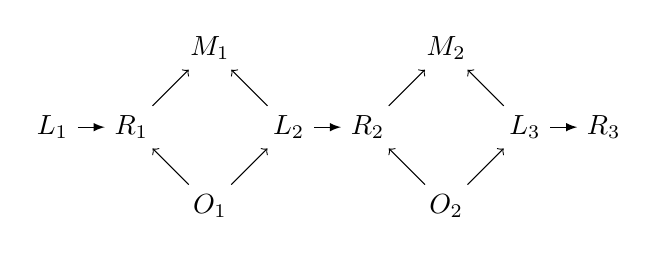
\begin{tikzpicture} %[scale=0.8]
  \node (o1) at (0,-1) {\(O_1\)};
  \node (m1) at (0,1) {\(M_1\)};
  \node (r1) at (-1,0) {\(R_1\)};
  \node (l1) at (-2,0) {\(L_1\)};
  \node (l2) at (1,0) {\(L_2\)};
  \node (r2) at (2,0) {\(R_2\)};
  \node (o2) at (3,-1) {\(O_2\)};
  \node (m2) at (3,1) {\(M_2\)};
  \node (l3) at (4,0) {\(L_3\)};
  \node (r3) at (5,0) {\(R_3\)};
  \draw [->] (o1) -- (r1);
  \draw [->] (o1) -- (l2);
  \draw [->] (r1) -- (m1);
  \draw [->] (l2) -- (m1);
  \draw [->] (o2) -- (r2);
  \draw [->] (o2) -- (l3);
  \draw [->] (r2) -- (m2);
  \draw [->] (l3) -- (m2);
  \draw [>=latex, ->] (l1) -- (r1);
  \draw [>=latex, ->] (l2) -- (r2);
  \draw [>=latex, ->] (l3) -- (r3);
\end{tikzpicture}
\]
We then apply the rewriting of $M_1$ using $r_2$ and combine the context with $M_2$ (this step is formally defined in~\autoref{def:seq_comb}):
\[
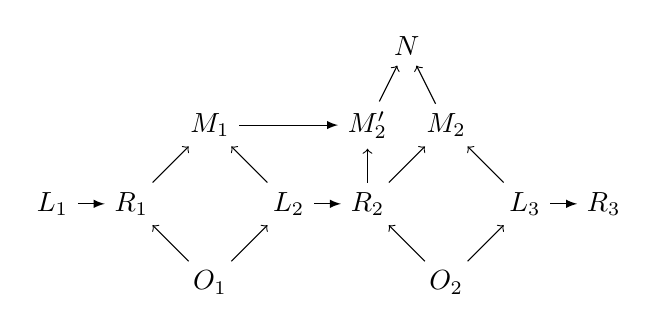
\begin{tikzpicture} %[scale=0.8]
  \node (o1) at (0,-1) {\(O_1\)};
  \node (m1) at (0,1) {\(M_1\)};
  \node (r1) at (-1,0) {\(R_1\)};
  \node (l1) at (-2,0) {\(L_1\)};
  \node (l2) at (1,0) {\(L_2\)};
  \node (r2) at (2,0) {\(R_2\)};
  \node (o2) at (3,-1) {\(O_2\)};
  \node (m2) at (3,1) {\(M_2\)};
  \node (l3) at (4,0) {\(L_3\)};
  \node (r3) at (5,0) {\(R_3\)};
  \node (m2p) at (2,1) {\(M_2'\)};
  \node (n) at (2.5,2) {\(N\)};
  \draw [->] (o1) -- (r1);
  \draw [->] (o1) -- (l2);
  \draw [->] (r1) -- (m1);
  \draw [->] (l2) -- (m1);
  \draw [->] (o2) -- (r2);
  \draw [->] (o2) -- (l3);
  \draw [->] (r2) -- (m2);
  \draw [->] (l3) -- (m2);
  \draw [->] (m2) -- (n);
  \draw [->] (m2p) -- (n);
  \draw [->] (r2) -- (m2p);
  \draw [>=latex, ->] (l1) -- (r1);
  \draw [>=latex, ->] (l2) -- (r2);
  \draw [>=latex, ->] (l3) -- (r3);
  \draw [>=latex, ->] (m1) -- (m2p);
\end{tikzpicture}
\]
We apply the rewriting steps on $N$ and obtain the refined sequence $N_0\action N_1\action N\action N_3$ (that we will formally introduce in~\autoref{def:propagate}):
\[
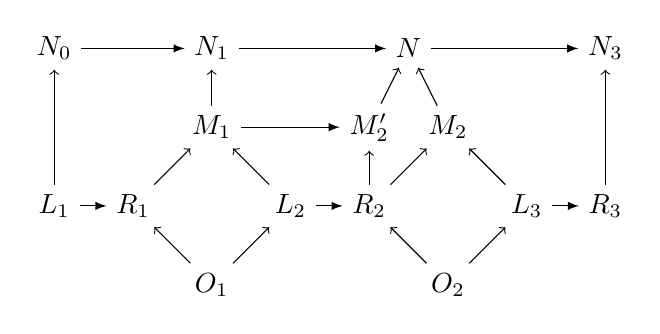
\begin{tikzpicture} %[scale=0.8]
  \node (o1) at (0,-1) {\(O_1\)};
  \node (m1) at (0,1) {\(M_1\)};
  \node (r1) at (-1,0) {\(R_1\)};
  \node (l1) at (-2,0) {\(L_1\)};
  \node (l2) at (1,0) {\(L_2\)};
  \node (r2) at (2,0) {\(R_2\)};
  \node (o2) at (3,-1) {\(O_2\)};
  \node (m2) at (3,1) {\(M_2\)};
  \node (l3) at (4,0) {\(L_3\)};
  \node (r3) at (5,0) {\(R_3\)};
  \node (m2p) at (2,1) {\(M_2'\)};
  \node (n) at (2.5,2) {\(N\)};
  \node (n0) at (-2,2) {\(N_0\)};
  \node (n1) at (0,2) {\(N_1\)};
  \node (n3) at (5,2) {\(N_3\)};
  \draw [->] (o1) -- (r1);
  \draw [->] (o1) -- (l2);
  \draw [->] (r1) -- (m1);
  \draw [->] (l2) -- (m1);
  \draw [->] (o2) -- (r2);
  \draw [->] (o2) -- (l3);
  \draw [->] (r2) -- (m2);
  \draw [->] (l3) -- (m2);
  \draw [->] (m2) -- (n);
  \draw [->] (m2p) -- (n);
  \draw [->] (r2) -- (m2p);
  \draw [->] (l1) -- (n0);
  \draw [->] (m1) -- (n1);
  \draw [->] (r3) -- (n3);
  \draw [>=latex, ->] (l1) -- (r1);
  \draw [>=latex, ->] (l2) -- (r2);
  \draw [>=latex, ->] (l3) -- (r3);
  \draw [>=latex, ->] (m1) -- (m2p);
  \draw [>=latex, ->] (n0) -- (n1);
  \draw [>=latex, ->] (n1) -- (n);
  \draw [>=latex, ->] (n) -- (n3);
\end{tikzpicture}
\]
Let us now integrate $e_4<e_3$ in the sequence. Let $R_4\lemb M_4\remb L_3$ be the cospan obtained from $\labl(e_4)\redl{+}_O\labl(e_3)$.
The concurrent contexts $M_4$ and $N$ combine using their common subpart $L_3$ (formally introduced in~\autoref{def:conc_comb}):
\[
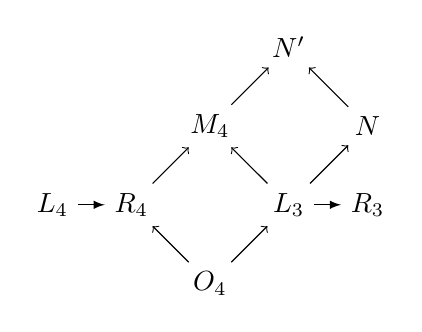
\begin{tikzpicture} %[scale=0.8]
  \node (l4) at (1,0) {\(L_4\)};
  \node (r4) at (2,0) {\(R_4\)};
  \node (o4) at (3,-1) {\(O_4\)};
  \node (m4) at (3,1) {\(M_4\)};
  \node (l3) at (4,0) {\(L_3\)};
  \node (r3) at (5,0) {\(R_3\)};
  \node (m2p) at (5,1) {\(N\)};
  \node (n) at (4,2) {\(N'\)};
  \draw [->] (o4) -- (r4);
  \draw [->] (o4) -- (l3);
  \draw [->] (r4) -- (m4);
  \draw [->] (l3) -- (m4);
  \draw [->] (m4) -- (n);
  \draw [->] (m2p) -- (n);
  \draw [->] (l3) -- (m2p);
  \draw [>=latex, ->] (l4) -- (r4);
  \draw [>=latex, ->] (l3) -- (r3);
\end{tikzpicture}
\]
Finally we propagate the context $N'$ to obtain
\[
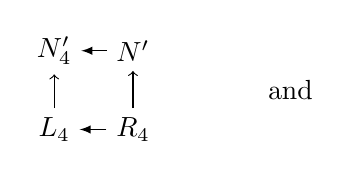
\begin{tikzpicture} %[scale=0.8]
  \node (l4) at (1,0) {\(L_4\)};
  \node (r4) at (2,0) {\(R_4\)};
  \node (n4) at (1,1) {\(N_4'\)};
  \node (m4) at (2,1) {\(N'\)};
  \node (and) at (4,0.5) { and };
  \draw [>=latex, ->] (r4) -- (l4);
  \draw [>=latex, ->] (m4) -- (n4);
  \draw [->] (r4) -- (m4);
  \draw [->] (l4) -- (n4);
\end{tikzpicture}
\qquad
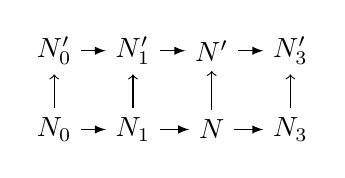
\begin{tikzpicture} %[scale=0.8]
  \node (n0) at (1,0) {\(N_0\)};
  \node (n1) at (2,0) {\(N_1\)};
  \node (n) at (3,0) {\(N\)};
  \node (n3) at (4,0) {\(N_3\)};
  \node (np0) at (1,1) {\(N_0'\)};
  \node (np1) at (2,1) {\(N_1'\)};
  \node (np) at (3,1) {\(N'\)};
  \node (np3) at (4,1) {\(N_3'\)};
  \draw [>=latex, ->] (n0) -- (n1);
  \draw [>=latex, ->] (n1) -- (n);
  \draw [>=latex, ->] (n) -- (n3);
  \draw [>=latex, ->] (np0) -- (np1);
  \draw [>=latex, ->] (np1) -- (np);
  \draw [>=latex, ->] (np) -- (np3);
  \draw [->] (n0) -- (np0);
  \draw [->] (n1) -- (np1);
  \draw [->] (n) -- (np);
  \draw [->] (n3) -- (np3);
\end{tikzpicture}
\]
The refinement of our story is then the set of transitions $N_0'\Rightarrow N_1'\Rightarrow N'\Rightarrow N_3'$ and $N_4'\Rightarrow N'$.

\end{example}

\begin{definition}[Refinement of a story]
  Given a story $s=(E,<)$ of graph rewriting events, define a refinement of $s$ as a sequence $(M_i\overset{m_i,p_i}{\Rightarrow} M_{i+1})_{e_i\in E}$,  such that there is a bijection $\imath$ between events $e\in E$ and transitions $M\overset{m,p}{\Rightarrow} M'$ which preserves label, i.e. $\labl(e)=p$ and such that for all $e_1,e_2\in E$, if $e_1<e_2$ and $\imath(e_1) = M_1\overset{m_1,p_1}{\Rightarrow} M_1'$, $\imath(e_1) =M_2\overset{m_2,p_2}{\Rightarrow} M_2'$ then $M_1'\iso M_2$.
\end{definition}

%Before giving the construction of a refinement $(M_i\overset{m_i,p_i}{\Rightarrow} M_{i+1})_{e_i\in E}$ let us first introduce some combinators of contexts.

\begin{definition}[Propagate a context]
  \label{def:propagate}
  Given a sequence $M_1{\Rightarrow} M_2\cdots {\Rightarrow} M_n\cdots {\Rightarrow} M_{m}$ and a graph $M_{n}'$ with $M_n\emb M_{n}'$ define the \emph{propagation} of $M_{n}'$ as the sequence  $M_1'{\Rightarrow} M_2'\cdots {\Rightarrow} M_n'\cdots {\Rightarrow} M_{m}'$ where
  \begin{itemize}
  \item $M_i'$, for $i<n$, is obtained by the reverse of the production $M_i\Rightarrow M_{i+1}$ applied to the new contexts;
  \item $M_i'$, for $n<i\leq m$, is obtained by the production $M_i\Rightarrow M_{i+1}$ applied to the new contexts.
  \end{itemize}
\end{definition}

\begin{definition}[Sequential combinator]
\label{def:seq_comb}
  Let $M_1\Rightarrow N_1$ and $M_2\Rightarrow N_2$ be two productions such that there exists $N_1\lemb R \remb M_2$ a cospan.
  Define $M_1\Rightarrow N_1\oplus_R M_2\Rightarrow N_2$ the productions $M_1'\Rightarrow M$ and $M\Rightarrow N_2'$, where $M$ is the pushout of the cospan $N_1\lemb R \remb M_2$ and $M_1'$, $N_2'$ are obtained by the propagation of $M$ to the two initial productions.
\end{definition}

\begin{definition}[Concurrent combinator]
\label{def:conc_comb}
  Let $M_1\Rightarrow N_1$ and $M_2\Rightarrow N_2$ be two productions such that there exists $N_1\lemb L \remb N_2$ a cospan.
  Define $M_1\Rightarrow N_1\otimes_L M_2\Rightarrow N_2$ the productions $M_1'\Rightarrow M$ and $M_2'\Rightarrow M$, where $M$ is the pushout of the cospan $N_1\lemb L \remb N_2$ and $M_1'$, $M_2'$ are obtained by the propagation of $M$ to the two initial productions.
\end{definition}

\begin{example}[Feedback loops]
Let us show how we can interpret negative feedback loops. Let $e_1\in s_1\redl{-} e_2\in s_2$ such that $s_2\subset s_1$. Then $e_2\leq_{s_1} e_2$. However this additional constraint does not change the way we interpret negative influence, that is the influence is realised if there exists $M$ such that the following diagram commutes:
\[
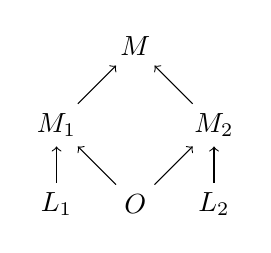
\begin{tikzpicture} %[scale=0.8]
  \node (o) at (0,0) {\(O\)};
  \node (n) at (0,2) {\(M\)};
  \node (l1) at (-1,0) {\(L_1\)};
  \node (l2) at (1,0) {\(L_2\)};
  \node (n1) at (-1,1) {\(M_1\)};
  \node (n2) at (1,1) {\(M_2\)};
  \draw [->] (l1) -- (n1);
  \draw [->] (l2) -- (n2);
  \draw [->] (o) -- (n1);
  \draw [->] (o) -- (n2);
  \draw [->] (n1) -- (n);
  \draw [->] (n2) -- (n);
\end{tikzpicture}
\]
\end{example}

Any refinement of a story into a trace is a potential \emph{concretisation} function. In our construction, we obtain a set of traces each representing possible concretisations for a story.

\begin{definition}[Concretisation of a poset]
  Given a set of posets $\mathcal{S}$ let us define the concretisation function $\gamma:\mathcal{S}\subseteq\Theta$ that sends a poset to a set of traces.
  \begin{itemize}
  \item
    Given a set of events $E$ and a labeling function $\labl$ on events, define a function $\mathit{decorate}:E\times E \to E\times E\times G$ that associates to a pair of events $(e,e')$ the following set
    \[
    \mathit{decorate}(e,e') = \{(e,e',O) : O\text{ is a graph such that }\labl(e)\redl{+}_O e'\}.
    \]

    Let $s = (E,<,\labl)$ be a poset. Define $\mathit{decorate}$ a function that sends a poset $s$ into a set of posets as follows
    \[
    \mathit{decorate}(E,<,\labl) =\{(E,\sqsubset,\labl) : e\sqsubset_O e' \iff (e,e',O)\in\mathit{decorate}(e,e')\text{ and }
    e<e'\}.
    \]
  \item Let $\overline{s}\in\mathit{decorate}(s)$ be a decorated poset. We define the refinement of a decorated poset into a trace $\mathit{refine}(\overline{s})$ as follows: for each pair of consecutive events $e \sqsubset_O e'$ construct the graph $G$ using the causal pair induce by $O$. Then propagate the graphs using the sequential and concurrent combinators.
  \end{itemize}
  The composition of the two functions $\gamma = \mathit{refine}(\mathit{decorate}(s))$ is the concretisation function.
\end{definition}

\begin{lemma}
  $\theta\subseteq \gamma(\alpha(\theta))$.
\end{lemma}
\begin{proof}
    \begin{mdframed}[backgroundcolor=blue!20]
    to do
  \end{mdframed}

\end{proof}

\subsection{Interpreting inhibition on stories}

In interpreting our logic, we work with a set of posets in $\mathcal{S}$ and a set of events $\cup_{s\in\mathcal{S}} E_s$.

\begin{definition}[Refinement of an event in a story]
  Let $e$ be an event in a story $s$. Let $t = M_1{\Rightarrow} M_2\cdots {\Rightarrow} M_n$ be a trace in $\gamma(\textit{infl}(s))$ and $\imath$ a bijection between $s$ and $t$.

  Define $\mathcal{R}(e\in s) = M$ such that $\imath(e) = M{\Rightarrow}M'$. We call such a graph $M$ a \emph{context of application} of $e$ in $s$.
\end{definition}


\begin{definition}[Refinement based on negative influence]
\label{def:ref_neg_infl}
  For two posets $s_1,s_2$ and two events $e_1\in s_1$ and $e_2\in s_2$ let the following be their refinements $\mathcal{R}(e_1\in s_1) = M_1$ and $\mathcal{R}(e_2\in s_2) = M_2$. Define $\mathcal{R}(e_1\in s_1\redl{-} e_2\in s_2) = M$ for which the diagram below commutes:
  \[
  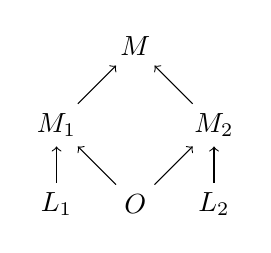
\begin{tikzpicture} %[scale=0.8]
    \node (o) at (0,0) {\(O\)};
    \node (n) at (0,2) {\(M\)};
    \node (l1) at (-1,0) {\(L_1\)};
    \node (l2) at (1,0) {\(L_2\)};
    \node (n1) at (-1,1) {\(M_1\)};
    \node (n2) at (1,1) {\(M_2\)};
    \draw [->] (l1) -- (n1);
    \draw [->] (l2) -- (n2);
    \draw [->] (o) -- (n1);
    \draw [->] (o) -- (n2);
    \draw [->] (n1) -- (n);
    \draw [->] (n2) -- (n);
  \end{tikzpicture}
  \]
  where $\labl(e_1)\redl{-}_O\labl(e_2)$.
\end{definition}
